\textbf{\underline{OZ 10 - De vergelijkingen van Maxwell - Oefening 5:}}
\vspace{0.5cm}

\begin{minipage}{.73\textwidth}
    Een lange cilindrische geleider met straal $R$ draagt een stroom $I$. De stroomdichtheid $J$ is niet uniform over de doorsnede van de geleider, maar variëert volgens $J = br$, met $b$ een positieve constante. Vind een uitdrukking voor het magnetisch veld $B$
    \begin{enumerate}[(a)]
        \item op een afstand $r_1 < R$,
        \item op een afstand $r_2 > R$.
    \end{enumerate}
\end{minipage}
\begin{minipage}{.23\textwidth}
    \begin{center}
        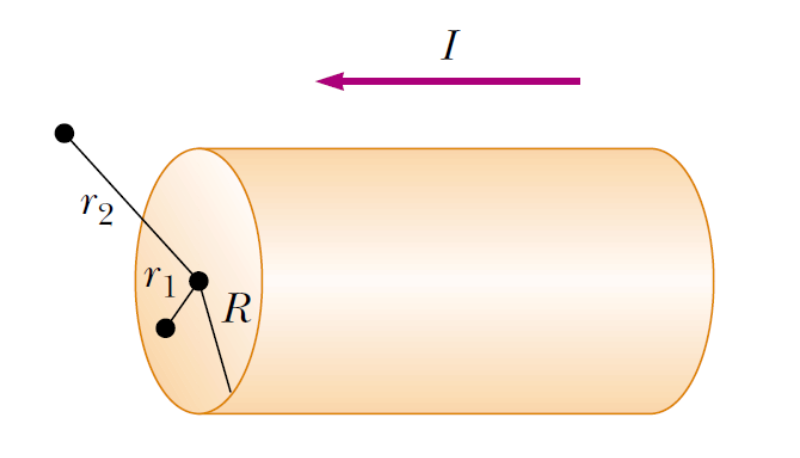
\includegraphics[scale = 0.4]{oz10/resources/Oz10Oef5.png}
    \end{center}
\end{minipage}

\begin{description}[labelwidth=1.5cm, leftmargin=!]
    \item[Geg. :]  $J = br$, $I$
\end{description}

\begin{enumerate}[(a)]
    \item 
        \begin{description}[labelwidth=1.5cm, leftmargin=!]
            \item[Geg. :]    $r_1 < R$
            \item[Gevr. :] $B_{\text{in}}$ ?
            \item[Opl. :]   
                De stroomdichtheid is niet uniform en varieert volgens $J = br$. De stroomdichtheid is de stroom per oppervlakte-eenheid, dus
                \begin{equation*}
                    I_{\text{in}} = \pi b r_1^3
                \end{equation*}
                waarbij b een postieve constante is. We passen de wet van Ampère toe op een cirkel met straal $r_1 < R$:
                \begin{align*}
                    \oint \vec{B} \cdot \vec{\ell} 
                        &= \mu_0 \pi r_1^2 br \\
                    B   &= \frac{\mu_0 br_1^2}{2}
                \end{align*}
        \end{description}
    \item
        \begin{description}[labelwidth=1.5cm, leftmargin=!]
            \item[Geg. :]   $r_2 > R$
            \item[Gevr. :] $B_{\text{uit}}$ ?
            \item[Opl. :]   
                Analoog aan (a) vinden we een stroom 
                \begin{equation*}
                    I_{\text{in}} = \pi b R^3.
                \end{equation*}
                We passen de wet van Ampère toe op een cirkel met straal $r_2 > R$:
                \begin{equation*}
                    B = \frac{\mu_0 b R^3}{2r_2}.
                \end{equation*}
        \end{description}
\end{enumerate}

\vspace{1cm}